\renewcommand{\lastmod}{September 22, 2023}
\renewcommand{\chapterauthors}{Markus Lippitz}

\chapter{Ray optics}



\goal{By the end of this chapter, you should be able to draw, calculate and align a ray's path through an optical system.}



\section{Overview}

I assume that you have seen a little bit of geometrical optics in your studies, but we will briefly review it. We will introduce the postulates of ray optics and discuss rays at a mirror and a lens as an example. I will also introduce the matrix method of ray optics, which is a very convenient way of calculating the path of a ray through a system of optical elements. More details on these topics can be found in chapter 1 of \cite{SalehTeich1991}, chapter 2 of \cite{Hering_Martin_Optik},  chapters 5 and 6 of \cite{Hecht_Optics}, chapter 2 of \cite{Konijnenberg_Optics}.


\section{Postulates of ray optics}

\paragraph*{Straight rays}  The propagation of light is described by straight rays that emerge from a source and end at a detector

\paragraph*{Index of refraction} A medium is described by its index of refraction $n$. The optical path length in a medium is given by the index of refraction $n$ times the geometric distance $d$. If $\br(s)$ describes a path in 3D space as a function of the path element $ds$, then the total optical path from A to B is
\begin{equation}
    \text{path length} = \int_A^B n(\br(s)) ds \quad .
\end{equation}

\paragraph*{Fermat's Principle} Of all the possible paths between points A and B, the light will take the one with the extremal (maximum or minimum) optical path length. This can be written as
\begin{equation}
    \delta \int_A^B n(\br(s)) ds  = 0
\end{equation}
and is Fermat's Principle. The $\delta$ means 'variation', i.e. you try to modify $\br(s)$ to find shorter (or longer) paths. If several paths have the same optical path length, then all of them are taken. Since the path length together with the velocity of light gives a travel time, and since one usually finds a minimum as an extremum, one can say that light travels along the path with the shortest travel time.

\section{Consequences of Fermat's Principle}
  
\paragraph*{Shadow} In an homogeneous medium the straight path is the shortest. A point source thus leads to a perfect projection of an aperture on a screen. 

\paragraph*{Mirror} At a mirror, the angle of incidence equals the angle of reflection, as this gives the shortest path. We can see this when we fold the reflected beam to the side behind the mirror. Then the point of reflection is the point where the ray would cross the mirror surface.


\paragraph*{Snell's law} At a bounday between two media ($i=1,2§$), the shortest path is such  that 
\begin{equation}
    n_i \sin \Theta_i = \text{const}
\end{equation}
where $n$ is the index of refraction and $\Theta$ the angle to tge surface normal. With our current model of ray optics, we can not say anything about the amplitude ratio of reflection and transmission at such an interface.


\section{Paraxial rays}

Before we look at some optical elements, we need to introduce the idea of a paraxial ray. All the optical elements we are going to look at have an axis of high symmetry, usually rotational symmetry. And in almost all cases the individual elements are placed one after the other, but on a common axis of symmetry. This axis is called the optical axis. The optical axis has a direction, which is typically the direction of the optical ray.

Paraxial rays are those that form only a small angle with the optical axis. This allows us to use the small angle approximation $\sin \theta \approx \theta$, which we will call paraxial approximation in this context. Optics under paraxial approximation is called Gaussian optics. Under paraxial approximation, spherical surfaces are good enough for imaging and focusing. Otherwise one would need aspheric surfaces, for example parabolic or elliptic shapes.


\section{Spherical boundary}

Before we come to a (spherical) lens, lets have a look at half a lens, i.e., a single spherical surface of radius $R$. For convenience, we encode in the sign of the $R$ the direction of curvature: a positive radius describes a convex surface, as seen when looking in the direction of the optical axis.

\begin{marginfigure}
    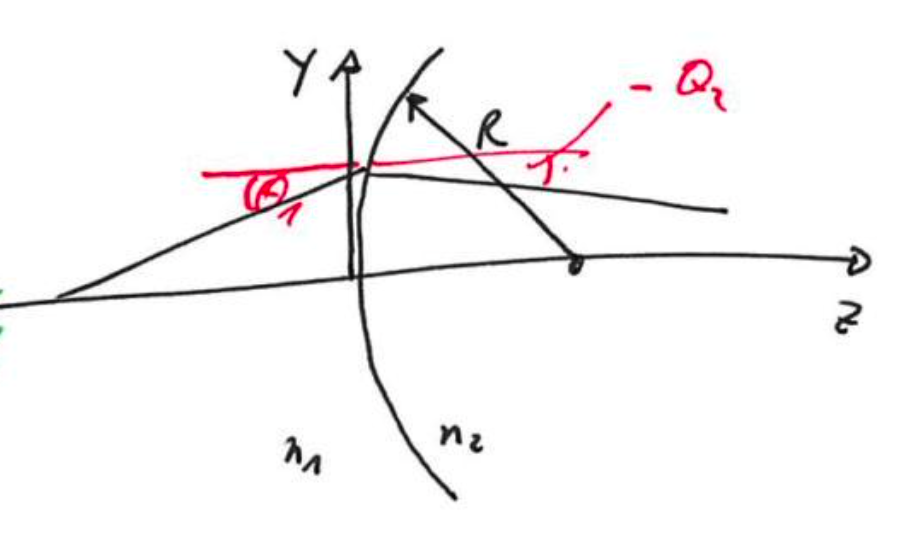
\includegraphics[width=\textwidth]{\currfiledir sketches/spherical_surface.png}
   \caption{Refraction of  a ray at a spherical surface}
\end{marginfigure}

We start with a ray of angle $\theta_1$ towards the optical axis in a medium of refractive index $n_1$. It hits the spherical surface at a height $y$ above the optical axis. Here we apply Snell's law and calculate the new direction of the ray. Using the paraxial approximation, we get
\begin{equation}
    \theta_2 \approx \frac{n_1}{n_2} \theta_1  \frac{n_2 - n_1}{n_2} \, \frac{y}{R}
    \label{eq:1_single_spherical_surface}
\end{equation}
Negative angles $\theta_i$ describe ray pointing towards below the optical axis.


We can do the same for many rays originating under different angles $\theta_1$ from  a point $P_1 =(y_1, z_1)$ in medium 1. We find that they all cross in a point $P_2 = (y_2, z_2)$ in medium 2. Point $P_1$ is thus imaged on point $P_2$. For convenience, the sign convention is thus that $z$ is measured from the intersection of the optical axis and the surface, i.e., both $z_i$ are positive.
We get
\begin{equation}
    \frac{n_1}{z_1} + \frac{n_2}{z_2} \approx \frac{n_2 - n_1}{R} \qquad 
    y_2 = - \frac{n_1}{n_2} \, \frac{z_2}{z_1} \, y_1
\end{equation}
The position $z_2$ along the optical axis of the image point does not depend on $y_1$, i.e., every point in the plane $z=z_1$ will have its image in the plane $z = z_2$. These two planes are \emph{conjugate planes}.




\section{Thin lens}

We combine two spherical surfaces of radius $R_1$ and $R_2$. In the sketch \ref{fig:1_thin_lens} $R_2$ is negative, as this is a concave surface when seen along the optical axis. The two surfaces enclose a medium of refractive index $n$, while the outside is air, i.e., $n_1 = 1$.

\begin{marginfigure}
    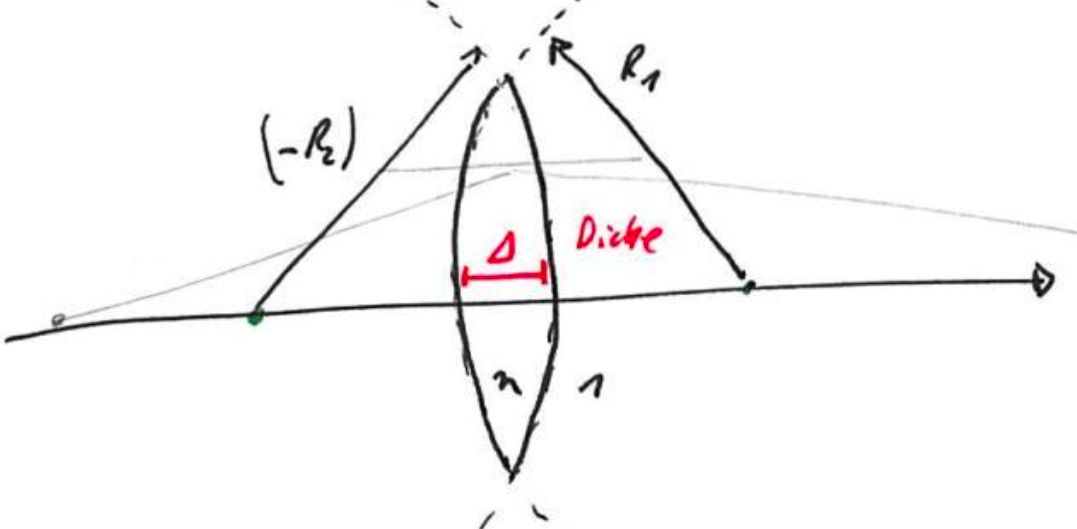
\includegraphics[width=\textwidth]{\currfiledir sketches/thin_lens.png}
   \caption{Refraction of  a ray at a thin lens}
   \label{fig:1_thin_lens}
\end{marginfigure}


We make the approximation that this is a \emph{thin lens}, i.e., that the width $\Delta$ of the lens on the optical axis is so small that we can neglect the change in height $y$ of the ray across the lens. We apply twice eq. \ref{eq:1_single_spherical_surface} and get
\begin{equation}
    \theta_2 = \theta_1 - \frac{y}{f} \quad \text{with} \quad
   \frac{1}{f} = (n-1) \left( \frac{1}{R_1} - \frac{1}{R_2} \right) \quad . 
\end{equation}
with the \emph{focal length} $f$. The coordinates of the image points are
\begin{equation}
    \frac{1}{z_1} + \frac{1}{z_2} = \frac{1}{f} \quad \text{and} \quad 
    y_2 = - \frac{z_2}{z_1} \, y_2
\end{equation}
Again, this holds only in the paraxial approximation. When the rays make a too large angle with the optical axis, they will not be focused ideally. A spherical lens shows aberrations.

\begin{marginfigure}
    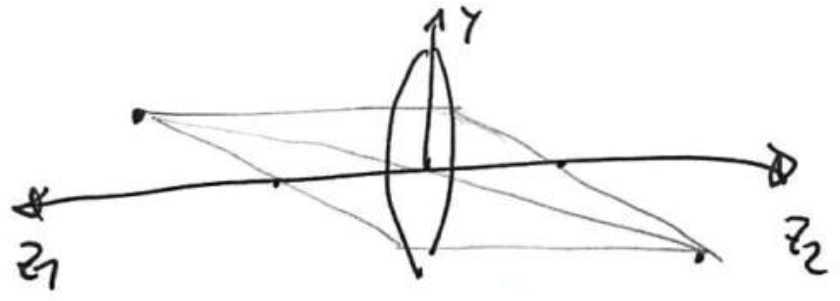
\includegraphics[width=\textwidth]{\currfiledir sketches/thin_lens_image.png}
   \caption{Image formation at a  thin lens}
   \label{fig:1_thin_lens_image}
\end{marginfigure}


For three special rays the action of a lens becomes very simple:
\begin{itemize}\setlength{\itemsep}{0pt}
    \item a ray that arrives parallel to the optical axis ($\theta_1 = 0$) will leave such that it passes through the focal point $(0,f)$ on the other side
    \item  a ray that arrives passing the  focal point will leave parallel to the optical axis
    \item a ray that passes through the center of the lens ($y = 0$) will remain unchanged
\end{itemize}
These rules have been formulated assuming a positive focal length $f$. When $f$ is negative, the same rules apply, but it  appears that the ray would have passed the  focal point on the other side of the lens. Additionally, it helps to remember that parallel rays will intersect in the focal plane.


\section{Matrix method}
When tracing a ray through an optical system, all you have to do is apply Snell's law at each interface. This is possible, but a bit tedious. A simpler approach is the idea of matrix optics. We describe a ray at a given position $z$ along the optical axis by two parameters: its angle $\theta$ with the optical axis and its height $y$ above the axis. We assume rotational symmetry so that $x=y$ and combine $\theta$ and $y$ into one vector. The effect of each optical element can then be written as a matrix acting on the vector, since in the paraxial approximation everything becomes linear.

\begin{marginfigure}
    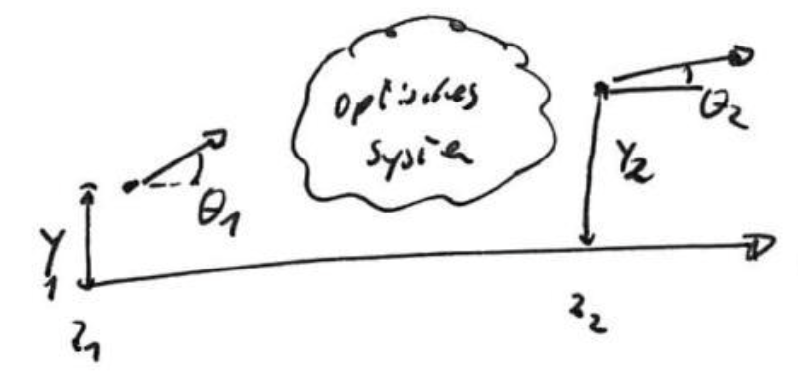
\includegraphics[width=\textwidth]{\currfiledir sketches/matrix_idea.png}
   \caption{The ray-transfer matrix describes the optical system between two planes.}
\end{marginfigure}

\paragraph*{Propagation} When a ray travels a distance $d$ through a homogeneous medium, its angle does not change. The height $y$ changes by $d \cdot \theta$. We write this as a ray-transfer matrix
\begin{equation}
    \begin{pmatrix}
        y_2 \\ \theta_2 
    \end{pmatrix}
    = 
    \boldsymbol{M}_\text{prop}
    \cdot
    \begin{pmatrix}
        y_1 \\ \theta_1 
    \end{pmatrix}
    \quad
    \text{with} \quad 
    \boldsymbol{M}_\text{prop} = 
    \begin{pmatrix}
        1 & d \\ 0 & 1
    \end{pmatrix} \quad .
\end{equation}

\paragraph*{Planar interface} Refraction at a planar interface does not change the height, but the angle
\begin{equation}
    \boldsymbol{M}_\text{planar} = 
    \begin{pmatrix}
        1 & 0 \\ 0 & \frac{ n_1 }{n_2}
    \end{pmatrix} \quad .
\end{equation}


\paragraph*{Spherical interface} Refraction at a spherical interface also does not change the height. The change in angle depends on ray height $y$
\begin{equation}
    \boldsymbol{M}_\text{spherical} = 
    \begin{pmatrix}
        1 & 0 \\ - \frac{n_2 - n_1}{n_2 R} &  \frac{ n_1 }{n_2}
    \end{pmatrix} \quad .
\end{equation}

\paragraph*{Thin lens} The action of a thin lens in paraxial apprixaltion is
\begin{equation}
    \boldsymbol{M}_\text{lens} = 
    \begin{pmatrix}
        1 & 0 \\ - \frac{1}{f} &  1
    \end{pmatrix} \quad .
\end{equation}


A sequence of optical elements is modelled as a product of ray transfer matrices. Note that the order is reversed. We typically propagate a ray from left to right, but mathematics is of Arabic origin, i.e. reads from right to left. The very first optical element is therefore represented by the rightmost matrix in the matrix product.

\section{Example: Point source in the focal plane of a lens }

As an example, let us calculate the effect of a point source that is placed in the focal plane of a thin lens. We start with a ray vector
\begin{equation}
\boldsymbol{v}_\text{in} = 
    \begin{pmatrix}
        y \\ \theta
    \end{pmatrix}  \quad , 
\end{equation}
let it propagate by a distance $d=f$ and then pass through a lens. In total we have
\begin{equation}
    \boldsymbol{v}_\text{out} = \boldsymbol{M}_\text{lens} \cdot  \boldsymbol{M}_\text{prop} \cdot \boldsymbol{v}_\text{in}
    = 
    \begin{pmatrix}
        y  + f \theta \\ - \frac{y}{f}
    \end{pmatrix}
\end{equation}
We see that the outgoing angle $\theta_\text{out} = - y/f$ does not depend on the direction $\theta$ in which the ray leaves the point source. All these rays are thus parallel, as expected.

\begin{marginfigure}
    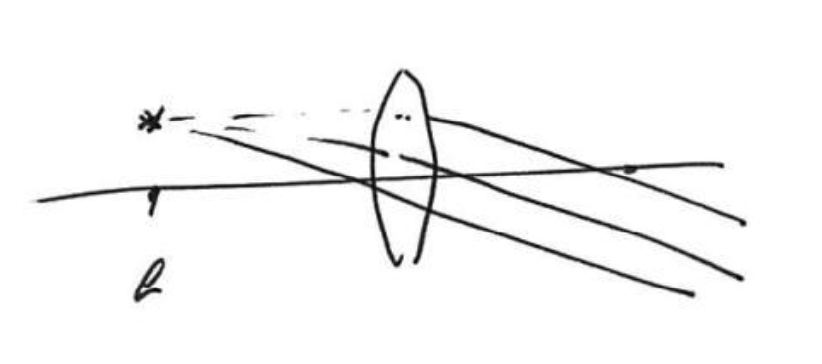
\includegraphics[width=\textwidth]{\currfiledir sketches/matrix_example.png}
   \caption{Point source in the focal plane of a lens }
\end{marginfigure}



\section{A thick lens with principal planes}

The approximation of a thin lens can be removed by introducing principal planes\sidenote{German: Hauptebenen}. It can be shown that the action of a thick lens (i.e, to spherical surfaces separated on the optical axis by a larger distance) and even the action of a sequence of lenses can be described as a single thin lens plus two principal planes. The rays enter the first principal plane and then immediately leave the second principal plane as if they would have passed an effective thin lens of focal length $f$. The position of the planes and the effective focal length are the only free parameters.


\begin{marginfigure}
    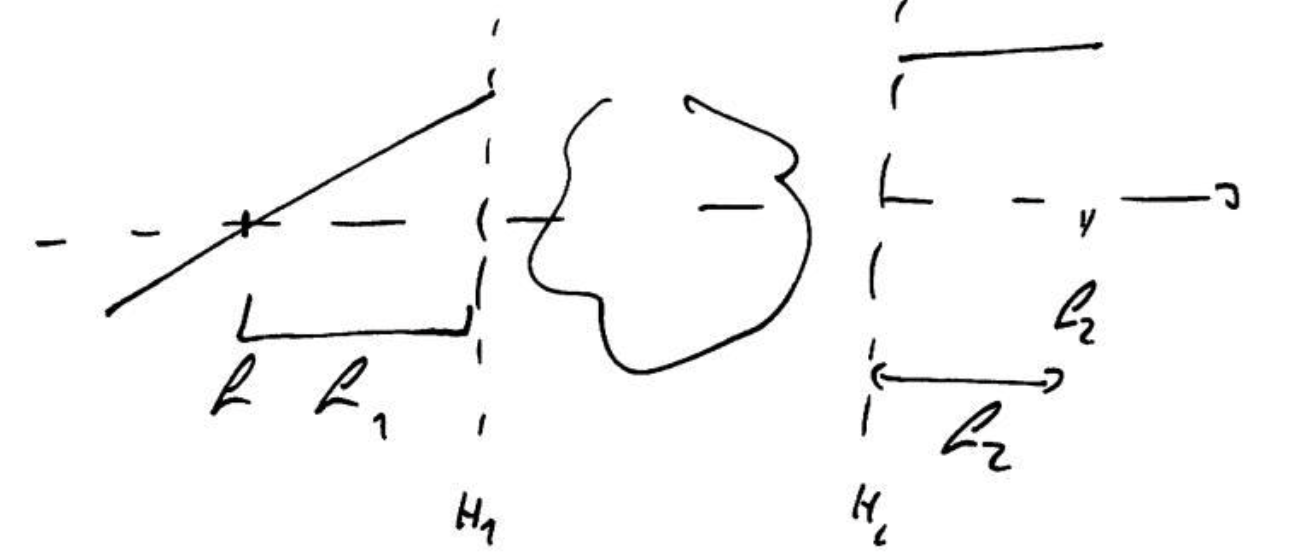
\includegraphics[width=\textwidth]{\currfiledir sketches/principal_plane.png}
   \caption{The two principal planes simplify many optical systems.}
\end{marginfigure}

\begin{questions}
\item A telephoto lens consists of many lenses, but can still be described by a single focal length. This focal length can be longer than the distance between the front lens and the film. The effective single lens is therefore outside the telephoto lens. This can be described by introducing principal planes in the matrix method of ray optics.
 
   Consider an optical element that can be described by a transfer matrix $\boldsymbol{M}$ with $\det(\boldsymbol{M}) = 1$. The two principal planes are located at distances $d_1$ before and $d_2$ after this element. These distances may also be negative. Assume that the refractive index of these domains is one. Show that these three domains together act like a thin lens and calculate $d_1$ and $d_2$.

\item  Show that any arrangement of thin lenses and distances between these lenses satisfies the above requirement $\det(\boldsymbol{M}) = 1$. \newline Hint: $\det(\boldsymbol{A} \boldsymbol{B} )  = \det(\boldsymbol{A})  \det(\boldsymbol{B}) $
\end{questions}


\subsection{Aberrations}
For\sidenote{This section is  adapted from \cite{Konijnenberg_Optics}} designing advanced optical systems Gaussian geometrical optics is not sufficient. 
Instead non-paraxial rays, and among them also non-meridional\sidenote{meridional rays run in a plane than contains the optical axis} rays, must be traced  using software based on Snell's Law with the sine of the angles of incidence and refraction. Often many thousands of rays are  traced to evaluate the quality of an image. 
It is then found that in general the non-paraxial rays do not intersect at the ideal Gaussian image point. Instead of a single spot, a spot diagram is found which is more or less confined. The deviation from an ideal point image  is quantified in terms of  \emph{aberrations}. One distinguishes between monochromatic and chromatic aberrations. The latter are caused by the fact that the refractive index depends on wavelength. The first are a consequence of the small angle approximation in paraxial optics. If instead one retains the first two terms of the Taylor series of the sine,  the errors in the image can be quantified by  five monochromatic aberrations, the so-called \emph{primary} or \emph{Seidel aberrations} (see, for example, wikipedia\sidenote{\url{https://en.wikipedia.org/wiki/Optical_aberration}}). The best known  is \emph{spherical aberration}, which is caused by the fact that for a convergent spherical lens, the rays that makes a large angle with the optical axis are focused closer to the lens than the paraxial rays (see Fig.~\ref{fig:1_Spherical_aberration}
). \emph{Distortion} causes deformation of images due to the fact that the magnification depends on the distance of the object point to the optical axis.



\begin{marginfigure}
  %  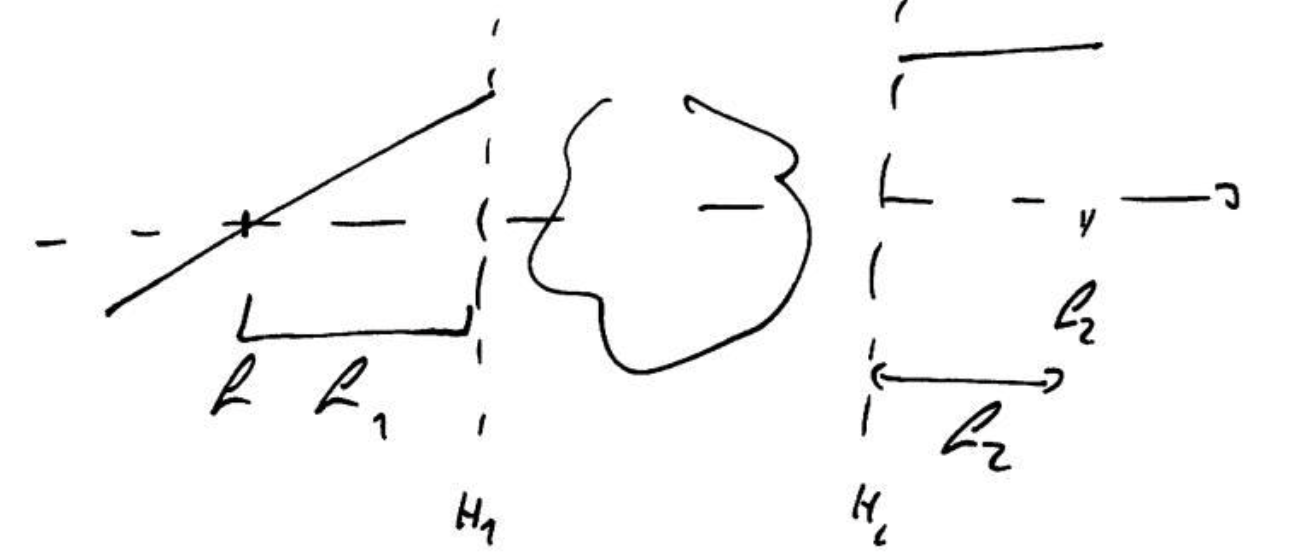
\includegraphics[width=\textwidth]{\currfiledir sketches/principal_plane.png}
   \caption{XXX spherical aberration}
\label{fig:1_Spherical_aberration}
\end{marginfigure}



For high-quality imaging the aberrations have to be reduced by adding more lenses and optimizing  the curvatures of the surfaces, the thicknesses of the lenses and  the distances between them. For high quality systems,  a lens with an aspherical surface is sometimes used.  Systems with very small aberrations are extremely expensive, in particular if the field of view is large, as is the case in  lithographic imaging systems used in the manufacturing of integrated circuits.




\section {Hands on: Aligning optical elements I}

In the practical part of this chapter, you should practice to align optical elements as mirrors, lenses and beam splitters.

\paragraph*{Laser beam} We will discuss in the next chapter the idea of a laser beam more iin detail. For now, it is sufficient to think of a bundle of rays that run more or less parallel to each other. So the beam is described by the diameter of the ray bundle and the angle of divergence within the bundle. Without lenses, we can for now assume that the rays remain parallel so that a laser beam can be approximated by a ray of geometrical optics.

\paragraph*{Degrees of freedom} It is useful to have in mind the degrees of freedom that a ray of light has. Above we have used $y$ $\theta$ to describe a ray in a single plane. In three dimensions, we need two spatial coordinates $x$ and $y$, and two angles with the optical axis, say $\theta_x$ and $\theta_y$. If we want to align and thus define a beam, we need to fix these four degrees of freedom.

\paragraph*{Alignment tip} A three-dimensional volume above an optical table is quite huge. In almost all cases it is not needed. It is sufficient to restrict the beam to one plane parallel to the table surface. The height of the beam above the table is defined by tje alignment tip. The center of the tip should coincide with the center of the beam.

\paragraph*{Defining the first leg} The laser beam leaves the laser typically in an not too well defined direction and position. We then need two mirrors to define the four degrees of freedom of the beam as each mirror is described by two angles. We place the tip first after the second mirror and use the first mirror to bring the beam on the tip. Then we place the tip far from the second mirror and use the second mirror for alignment. Iterating this procedure will converge.\sidenote{The other way round does not converge!}

\paragraph*{Defining all further legs} The advantage of a fixed beam hight comes with all further legs of the beam path. At a third mirror, the beam has already the correct height. We place the mirror such that its surface sits at the intersection oif the first two legs. Then we use the two angles of the mirror to define the new direction of tge beam.

\paragraph*{Lenses} A lens should be centered on the beam. We first align the beam without lens, then place the tip after the intended position of the lens. We put the lens into the beam and translate perpendicular to the beam until it again goes over the tip. The angle of the lens relative to the beam can be check by back reflections. When translating the lens in beam direction, one needs to pay attention that the lens does not leave its centered position.

\paragraph*{Beam splitter} At a beam splitter, three rotational degrees of freedom come into play. The translational degrees are identical with those of a mirror.






%--------------------
\printbibliography[segment=\therefsegment,heading=subbibliography]
